\documentclass{article}

\usepackage[a4paper, total={6in, 9in}]{geometry}
\usepackage{tikz}
\usepackage{gensymb}
\usetikzlibrary{shapes.geometric, arrows}

%Flowchart Setup
\tikzstyle{boxes} = [rectangle, minimum width=2cm, minimum height=1cm, text centered, text
width=2cm, draw=black]
\tikzstyle{arrow} = [thick, ->, >=stealth]
\tikzstyle{infobox} = [trapezium, trapezium left angle=70, trapezium right angle=110, minimum
width=2cm, minimum height=1cm, text centered, text width=2cm, draw=black]

\title{Brad Flavall Guest Lecture Summary}

\author{Jos Craw\\35046080}

\begin{document}

\maketitle{}

Brad's lecture was on industry structure. He works at Beca where he worked on an indoor substation
in Christchurch. First Brad talked about the New Zealand power distribution network and its
various stages.\\

\begin{figure}[h]
%Drawing flowchart
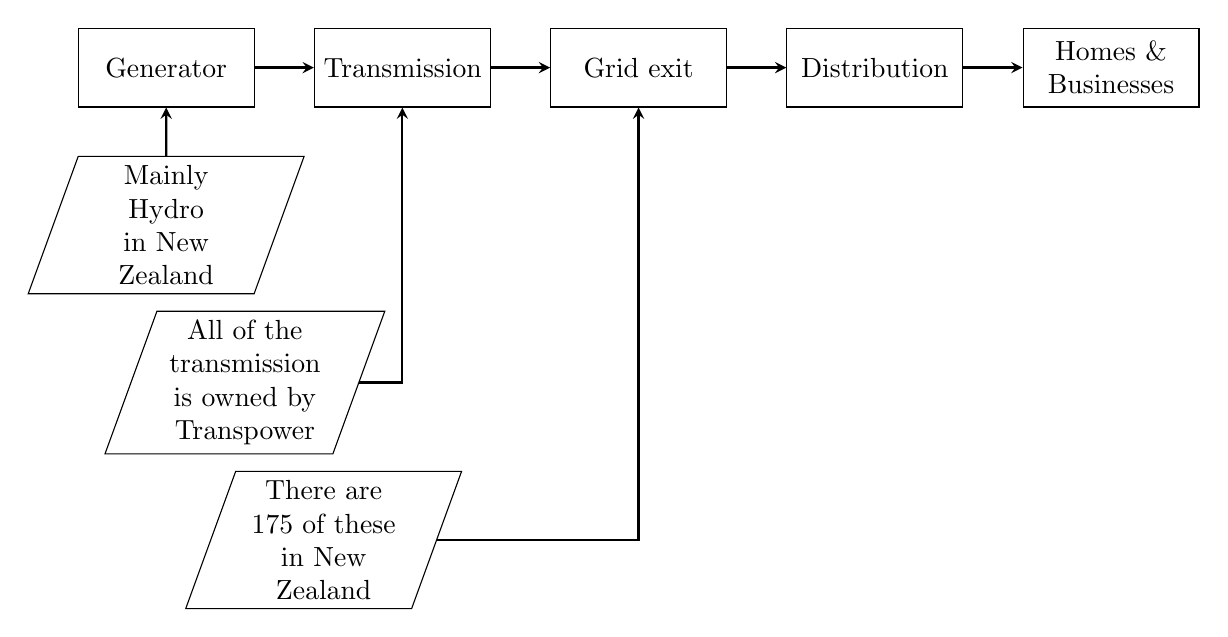
\begin{tikzpicture}
    %Main Nodes
    \node (gen) [boxes] {Generator};
    \node (trans) [boxes, right of=gen, xshift=2cm] {Transmission};
    \node (gridEx) [boxes, right of=trans, xshift=2cm] {Grid exit};
    \node (dist) [boxes, right of=gridEx, xshift=2cm] {Distribution};
    \node (output) [boxes, right of=dist, xshift=2cm] {Homes \& Businesses};

    %Supplementary Nodes
    \node (genInfo) [infobox, below of=gen, yshift=-1cm] {Mainly Hydro in New Zealand};
    \node (transInfo) [infobox, below of=trans, right of=genInfo, yshift=-1cm] {All of the
        transmission is owned by Transpower};
    \node (gridExInfo) [infobox, below of=gridEx, right of=transInfo, yshift=-1cm] {There are 175 of these in New Zealand};

    %Arrows
    \draw [arrow] (gen) -- (trans);
    \draw [arrow] (trans) -- (gridEx);
    \draw [arrow] (gridEx) -- (dist);
    \draw [arrow] (dist) -- (output);
    \draw [arrow] (genInfo) -- (gen);
    \draw [arrow] (transInfo) -| (trans);
    \draw [arrow] (gridExInfo) -| (gridEx);
    
\end{tikzpicture}
\caption{The New Zealand power distribution network}
\end{figure}

The next item that brad discussed was the statistics for New Zealand energy usage. New Zealanders
use 27\% of their energy on heating, 17\% on refrigeration, 13\% on lighting, and 3\% on drying.\\ 

The next topic discussed was the seasonal effects on the Transpower grid. These changes can be
observed in the winder when the area on the Alps increases energy usage dramatically. These
changes can be due to population shift and seasonal changes such as weather. This causes lots of
strain on the grid however, none of the major companies wants to do anything. This is because
upgrading the grid is very expensive and there is no huge benefit to the company that upgrades 
versus all other suppliers.\\

Brad then moved on to the design and construction of the indoor Christchurch substation. Brad
talked about some facts about the process for adding this substation. The design took 20,000+
hours to construct, with 86 people. The design itself took 4,800 design hours. Brad talked about
the complexity of design and the coordination between many different engineering disciplines, such
as electrical, structural and coordination with the local council to build the design.\\

Brad next went over the difficulties and potential issues encountered. The first was that the
pipes under the transformer were bent at 90\degree this issue was found one day before concrete
was poured. The angle was changed to a shallower one to allow the cable to be routed through.\\

Brad then talked about the benefits of the addition of this new substation. As there used to be
only one substation for Christchurch when an issue occurred with it much of the electricity failed
but with this new substation redundancy was introduced, this allowed one of the substations to
have issues and the grid remain functional.
\end{document}
